%!TEX root = ../Main.tex

\section{Evaluation}
\label{s:Evaluation}

\TODO{Discuss the performance of the system. Why this is a good idea. Give graphs that show the number of states is sensible when more processes are fused in.}


\subsection{Optimisation}
\label{s:Optimisation}
After the algorithm has completed fusing both processes it may be possible to eliminate redundant @jump@, depending on how the affected variables are used by other instructions.

\TODO{Discuss combining jump instructions here. Use this to motivate the need for drop instructions.}

\begin{figure}

% I thought these two looked nicer separately, but let me know if you want them in a single graph
\begin{minipage}[t]{0.4\textwidth}
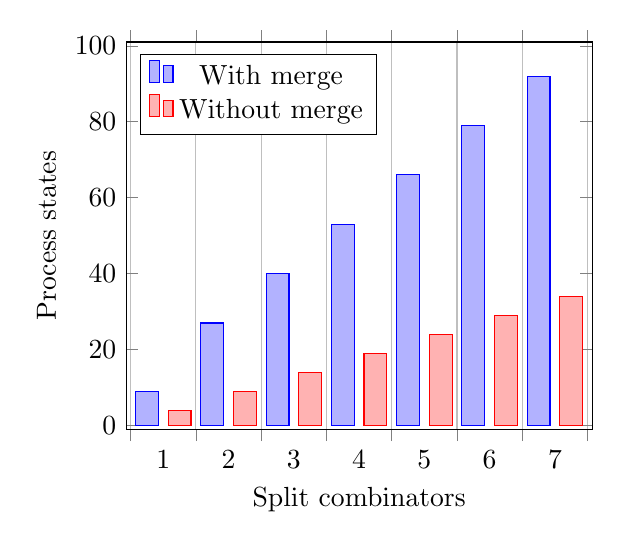
\begin{tikzpicture}
\begin{axis}[
	ylabel=Process states,
	xlabel=Split combinators,
  ymin=0, ymax=100,
	enlargelimits=0.01,
	ybar interval=0.7,
  width=7.5cm, height=6.5cm,
	legend pos=north west,
]
\addplot coordinates {(1,9) (2,27) (3,40) (4,53) (5,66) (6,79) (7,92)
  % Last bar doesn't show for some reason, so need to add a dummy value for the next one
    (8,1) };

\addplot coordinates {(1,4) (2,9) (3,14) (4,19) (5,24) (6,29) (7,34)    (8,1) };

\legend{With merge, Without merge};

\end{axis}
\end{tikzpicture}
\end{minipage}
\begin{minipage}[t]{0.10\textwidth}
\quad
\end{minipage}
\begin{minipage}[t]{0.4\textwidth}
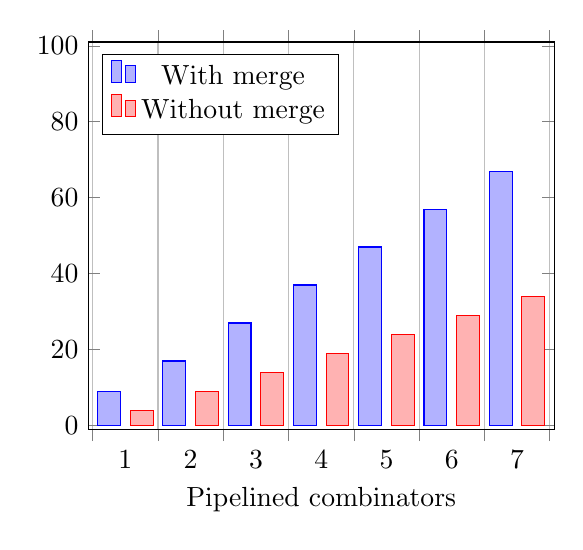
\begin{tikzpicture}
\begin{axis}[
% Hide the label on the second graph
%	ylabel=Process states,
	xlabel=Pipelined combinators,
  ymin=0, ymax=100,
	enlargelimits=0.01,
	ybar interval=0.7,
  width=7.5cm, height=6.5cm,
	legend pos=north west,
]
\addplot coordinates {(1,9) (2,17) (3,27) (4,37) (5,47) (6,57) (7,67)   (8,1) };

\addplot coordinates {(1,4) (2,9) (3,14) (4,19) (5,24) (6,29) (7,34)    (8,1) };

\legend{With merge, Without merge};

\end{axis}
\end{tikzpicture}
\end{minipage}

\caption{Maximum output process size for fusing all combinations of up to $n$ combinators.}
\label{fig:bench:outputsize}
\end{figure}


\begin{figure}

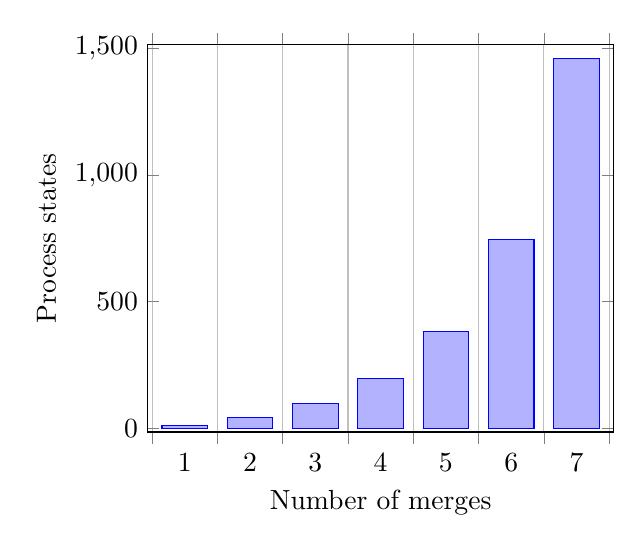
\begin{tikzpicture}
\begin{axis}[
	ylabel=Process states,
	xlabel=Number of merges,
%  ymode=log,
  ymin=0, ymax=1500,
	enlargelimits=0.01,
	ybar interval=0.7,
  width=7.5cm, height=6.5cm,
	legend pos=north west,
]
% These are the values for splitting.
% They are smaller than the 'chaining', but look much nicer on the linear graph.
\addplot coordinates {(1,9) (2,42) (3,97) (4,196) (5,383) (6,746) (7,1461)
  % (8,2880)
  (8,1)
  };

% These are the values for chaining
% \addplot coordinates {(1,4) (2,48) (3,194) (4,760) (5,2814) (6,10064) (7,1) };

\end{axis}
\end{tikzpicture}

\caption{Exponential blowup occurs when splitting or chaining merges together.}
\label{fig:bench:exponential}
\end{figure}

